\section{Data}\label{sec:data}

\subsection{Loans}

The loan data are Freddie Mac's Single-Family Loan-Level Dataset, Standard
Dataset, Release 47 \citep{FreddieGuide2026}: fully amortizing, full-documentation
fixed-rate mortgages Freddie Mac acquired with a first payment from 1999 to
mid-2026, with monthly performance through June 2026. The standard dataset is
a subset of Freddie Mac's book: it excludes, among others, adjustable-rate,
interest-only and government-insured loans, affordable-housing products other
than Home Possible loans funded from March 2015, and loans with credit
enhancement other than primary mortgage insurance. ``Freddie Mac's book''
below means this standard subset.
For each origination quarter there is one origination file and one monthly
performance file; the \num{data.quarters} quarters hold \num{data.orig_rows}
loans and \num{data.perf_rows} billion loan-months. The terms of use allow publishing
noncommercial research results and derived products that cannot be used to
recreate the data \citep{FreddieTerms2025}. The repository therefore releases code and aggregate
results only; no loan-level file leaves the author's machine.

The ingest checks, on every quarter, that each record has the documented
number of fields, that loan identifiers are well formed and unique, that every
performance record belongs to a loan in the matching origination file, that no
loan has two records for the same month, and that every loan is fixed-rate.
All checks pass. \Cref{tab:flow} gives the sample flow. Loans in Puerto Rico,
Guam and the U.S. Virgin Islands, and one loan with no state (\num{data.excl_hpi}
in all), are dropped because the state house-price and unemployment series do
not cover them, as are
\num{data.excl_ltv} loans with no original LTV, whose property value is
therefore unknown.

\begin{table}[t]\centering\small
\caption{Sample flow.}\label{tab:flow}
\begin{tabular}{lr}\toprule
Loans in the 110 origination files & 49{,}483{,}298 \\
\quad without any performance record & 293 \\
\quad outside the 50 states and DC (one with no state) & 74{,}879 \\
\quad no original LTV & 1{,}853 \\
\quad no original interest rate & 0 \\
Loans kept & 49{,}406{,}273 \\
\quad active at one or more year-ends (in the panel) & 47{,}099{,}933 \\
Loan-years with an outcome{,} December 1999--2024 & 221{,}415{,}514 \\
Loan-years censored and dropped (defect or reperforming-sale removal) & 111{,}612 \\
Loans active at December 2025 (last portfolio) & 13{,}073{,}255 \\
\bottomrule\end{tabular}
\end{table}


\Cref{fig:data} shows the book and its outcomes. The active book grows from
about one million loans at the end of 1999 to \num{data.active_2025} million
at the end of 2025. Annual default rates peak at \num{data.dr_peak_gfc}\% in
\num{data.dr_peak_gfc_year} and again at \num{data.dr_2020}\% in 2020. The
2020 spike is the pandemic: loans in forbearance were reported delinquent by
contract, so many crossed 180 days. Their endings differ from the crisis
defaults. By June 2026, \num{data.ce_2009}\% of the loans that defaulted in
2009 had ended in a credit event, against \num{data.ce_2020}\% of those that
defaulted in 2020. Of the 2020 defaults, \num{data.po_2020}\% had been paid off
and \num{data.act_2020}\% were still active. The design's default definition
counts them as defaults, and the severity model counts their payoffs as
zero-loss resolutions.

\begin{figure}[t]
\centering
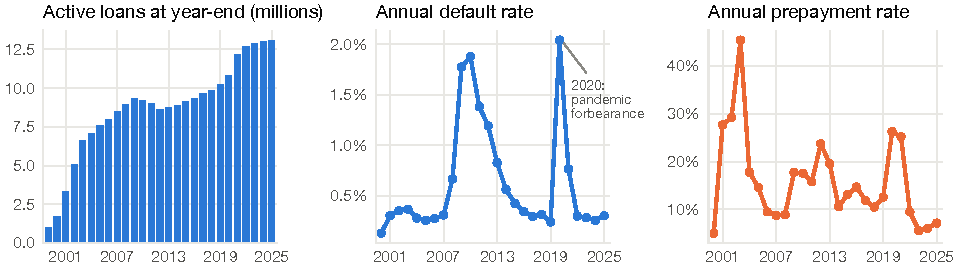
\includegraphics[width=\linewidth]{figures/data.pdf}
\caption{The Freddie Mac standard book. Left: loans active at each year-end.
Middle and right: share of active loans that default or prepay in the
following calendar year (default: first month 180+ days delinquent or a
credit-event zero balance).}
\label{fig:data}
\end{figure}

\subsection{Macro series}

House prices are the FHFA all-transactions index by state (FRED series
\texttt{\{ST\}STHPI}, quarterly), unemployment the BLS rate by state
(\texttt{\{ST\}UR}, monthly, seasonally adjusted), both for the 50 states and
the District of Columbia, and the market mortgage rate is Freddie Mac's PMMS
30-year fixed rate (\texttt{MORTGAGE30US}). A loan's origination month is
taken as two months before its first payment, because mortgage interest is
paid in arrears. The input at December $y$ uses the fourth-quarter index and
the December unemployment rate. Both are published in the first quarter of
$y+1$, before a December allowance is finalised. The checksums of the
downloaded series are in the repository.

\subsection{Judicial foreclosure}

Judicial-foreclosure states (Connecticut, Delaware, Florida, Iowa, Illinois,
Indiana, Kansas, Kentucky, Louisiana, Maine, North Dakota, New Jersey, New York,
Ohio, Pennsylvania, South Carolina, Vermont and Wisconsin) are those listed in
Table~2 of \citet{gerardi2013borrower}, whose assignment follows
\citet{rao2009foreclosing}. Foreclosure takes longer in these states. In the
severity tables (\cref{app:lgd}), judicial-state severity is the higher in
\num{data.jud.higher} of the \num{data.jud.n} band-and-date comparisons where
both cells have thirty or more resolutions; the exceptions are bands of 80\%
current LTV and above in 2008 to 2011.
